\chapter{绪论}
\section{课题来源与意义}
近几年来,随着互联网(Internet)的兴起和发展,互联网上积累的数据呈现急剧膨胀的态势。根据国际数据信息公司\footnote{https://www.idc.com/}(International Data Corporation, IDC)的统计和预测,2018~年全球网络数据量已经达到~1.8~ZB,预计到~2025~年,全球网站数据累积总量还将增长约~50~倍。
随着这类文本、视频、图像无标注的数据(Unlabeled Data)的大量涌现,如何利用现有的机器学习算法(Machine Learning),从这类已存在的大量的无标注数据中学习内在规律和知识以提取出有用的信息,已经变成了一个重要的挑战\upcite{王建翔2017面向可读性评估的词向量技术研究及实现}。
自从2006 年,以~Geoffrey Hinton~为代表的学者们提出的深度学习(Deep Learning, DL)理念~\upcite{hinton2006reducing}以来,这一新的思路为解决如何利用爆炸的数据量,以提取有效知识带来了新的前景。
在这之后的发展中,基于神经网络(Neural Network,NN)的表示学习技术(Representation Learning)开始快速拓展到各个相关研究领域中去。
尤其在图像分类(Image Classification)、语音自动识别(Automatic Speech Recognition,ASR)~\upcite{DBLP:journals/taslp/WangW16}和神经机器翻译(Neural Machine Translation,NMT)~\upcite{bahdanau2014neural}领域的多个任务上,基于深度模型的方法,在精确度和效率上远远超过了基于特征提取(Feature Extraction)的传统方法。

随着应用领域的拓展,深度学习技术逐渐在自然语言处理中(Natural Language Processing, NLP)得到广泛应用。 例如,蒙特利尔大学教授 Yousha Bengio 提出用神经网络来训练语言模型(Language Model,LM),并对模型中的各个结构细节进行了相关探索\upcite{DBLP:conf/nips/BengioDV00}。因为输入的维度是固定的N个单词的词向量,而不是动态长度,所以该方法不能有效处理单词的长距离单词依赖问题。
针对这个问题,在后续的工作中,由其学生~Tomas Mikolov~提出了采用循环神经网络(Recurrent Neural Network, RNN)\upcite{DBLP:journals/cogsci/Elman90}对上下文信息作为建模策略的方法,并逐步将该理论进行了拓展和简化\upcite{DBLP:conf/interspeech/MikolovKBCK10}。
循环神经网络主要特点是能够记忆该单词之前的所有出现过的单词的信息,即所谓的全局上下文信息(Global Context),用来预测下一个单词出现的对数概率分布。
因为RNN模型在训练过程中学习到了单词的前面出现的所有词,所以句子的长距离依赖关系(Long Term Dependency)可以被学习到,所以该方法在建模理论上克服了最初的神经网络语言模型的无法利用语句长距离上下文依赖的缺点。
另外,在模型训练的过程中,语义相似的单词被映射到的某低维子空间中,也满足了单词的语义相似(Semantic Similarity)的要求。相比统计语言模型(Statistical Language Model)领域中的N-gram模型,他不需要平滑技术(Smoothing Technology)来对文本中出现次数少的单词做处理。
到目前为止,RNN~模型已经演变出各种结构,应用在非常多的文本任务上面,并且都能取得了较为满意的结果。

由于RNN网络的计算时间与句子的平均长度正相关,所以基于~RNN~建模的算法计算时间都很大,需要更长的时间收敛。同时,我们需要看到最简单的RNN模型所使用的参数数量是NPLM模型的两倍多,这也意味着RNN模型需要占用更大的内存空间,消耗了更多的计算资源,导致其无法广泛应用到现实场景中去。
在文献~\cite{DBLP:conf/icassp/MikolovKBCK11}~中,Tomas Mikolov 提出了多种优化策略来消除该模型的各种缺点,例如:缩短模型求导步数、对词表(Vocabulary)做分解~\upcite{DBLP:journals/coling/BrownPdLM92}等策略,这些计算策略能保证模型的计算精度,同时极大提高了RNN网络的运算效率。

\section{国内外研究现状}
语言模型可以用来估算一段文序列组合的可能性,该模型在机器翻译(Machine Translation)、语音识别(Speech Recognition)等任务上都有着极为重要的作用。考虑到语言模型的漫长的发展历史,我们可以划分为两个主要阶段:统计语言模型(Statistical Language Model)和神经网络语言模型(Neural Language Model)。
其中,统计模型指代的是~N-gram~语言模型,而随着深度学习的爆发,各种神经网络语言模型变体逐渐发展并占据了主导地位。我们接下来会对这两个演化阶段所涉及的算法一一介绍。

\subsection{N-gram 语言模型}
首先介绍传统的~N-gram~语言模型,该算法属于典型的基于稀疏表示(Sparse Representation)的语言模型,因为一个单词表示方式是独热表示(One-Hot Representation)。该传统模型的意义不仅是提供了一种文本建模策略,而且定义了如何评价语言模型的好坏,并且定义了语言模型所涉及的相关拓展方向。

接下来给出~N-gram~统计语言模型的形式化定义。假设给定一个长度为$m$ 的单词字符串,$w_1$ 到$w_m$ 依次表示这段文本中的各个单词,我们需要求解一个概率分布$p(w_1,\cdots,w_m)$,以表示该字符串存在或者出现的可能性。在求解过程中,我们通常使用链式法则(Chain Rules),将计算整个序列概率问题分解成如下形式:
\begin{equation}
\setlength{\abovedisplayskip}{6pt}
\setlength{\belowdisplayskip}{6pt}
\label{equ:lm}
p(w_1,\cdots,w_m) =p(w_1)\prod_{t=1}^{m}p(w_t|w_1,\cdots,w_{t-1})
\end{equation}
在实际求解过程中,如果文本的长度较长,公式~(\ref{equ:lm})~中右部~$p(w_m | w_1,w_2,\cdots,w_{m-1}) $ 的估计误差会很大。因此,提出了~N~元模型(N-gram model),它能简化了实际问题的复杂度,最早被用来估算条件概率。需要注意的是,单词距离大于$n$单词会被直接忽略,该模型可以写成如下形式:
\begin{equation}
\setlength{\abovedisplayskip}{6pt}
\setlength{\belowdisplayskip}{6pt}
\label{equ:approx}
p(w_i | w_1,w_2,\cdots,w_{t-1})  \approx p(w_i | w_{t-(n-1)},\cdots,w_{t-1})
\end{equation}
假若~$n=1$~,此时称其为一元模型(Uni-gram model),公式~(\ref{equ:approx})~将会退化成~$p(w_i),i\in [1,n-1]$.此时,整个句子的概率计算公式为:~$p(w_1,w_2,\cdots,w_m) = p(w_1)p(w_2) \cdots p(w_m)$。
从这个退化的公式中,可以得知:在一元模型中,整个文本的概率是出现的各个单词的词频概率的乘积,它直接丢失了文本词组之间的顺序信息。当~$n = 2$~时,称为二元模型(Bi-gram model),公式~(\ref{equ:approx})~将会退化为 $p(w_t|w_{t-1})$。除此之外,还有 $n=3$ 时的三元模型(Tri-gram model),使用$p(w_t |w_{t-2},w_{t-1})$ 作为近似概率分布。当~$n>1$~的模型均可以保留一定的词序信息。

传统方法采用单词或者n元组的词频来作为n元组的概率计算方法,该方法简单有效能满足线上负载的计算需求。但是随着n的增大,模型的参数呈现指数爆炸式增长、概率计算复杂度也相应上升。目前谷歌有在线存储的最大的~9~元模型(Google N-gram Viewer)\footnote{https://books.google.com/ngrams},这已经是目前计算机系统存储,数据访问的极限了。


神经网络的建模思路源自于~N-gram~模型,它主要解决的问题是如何对文本的上下文信息利用先用的模型进行建模。历史上的模型,我们可以主要划分为:传统前向传递神经网络(Feed Forward Neural Network, FFNN)、循环神经网络(Recurrent Neural Network, RNN)以及双线性模型(Bilinear Model)这三种建模方案。 以下我们将一一探讨。


\subsection{前馈神经网络语言模型}
由于神经网络对参数进行高度共享,因此对低频词具有天然的平滑能力。这里所指的神经网络语言模型(Neural Probabilistic Language Model, NPLM) ,最早由Bengio等人在2001年提出\upcite{DBLP:conf/nips/BengioDV00}, 近年来一些学者开始展开这方面的研究,并取得一系列成果,如~\cite{DBLP:conf/acl/BaroniDK14,DBLP:journals/sigkdd/BellK07,DBLP:journals/pami/BengioCV13,DBLP:journals/tnn/BengioSF94}~。 但总体而言, 对NPLM的研究还处在起步阶段。具体而言,NPLM通过一个多层感知网络(Multi-Layer Perceptron, MLP)来计算公式~(\ref{equ:approx})~中概率。
\begin{figure}
  \centering
  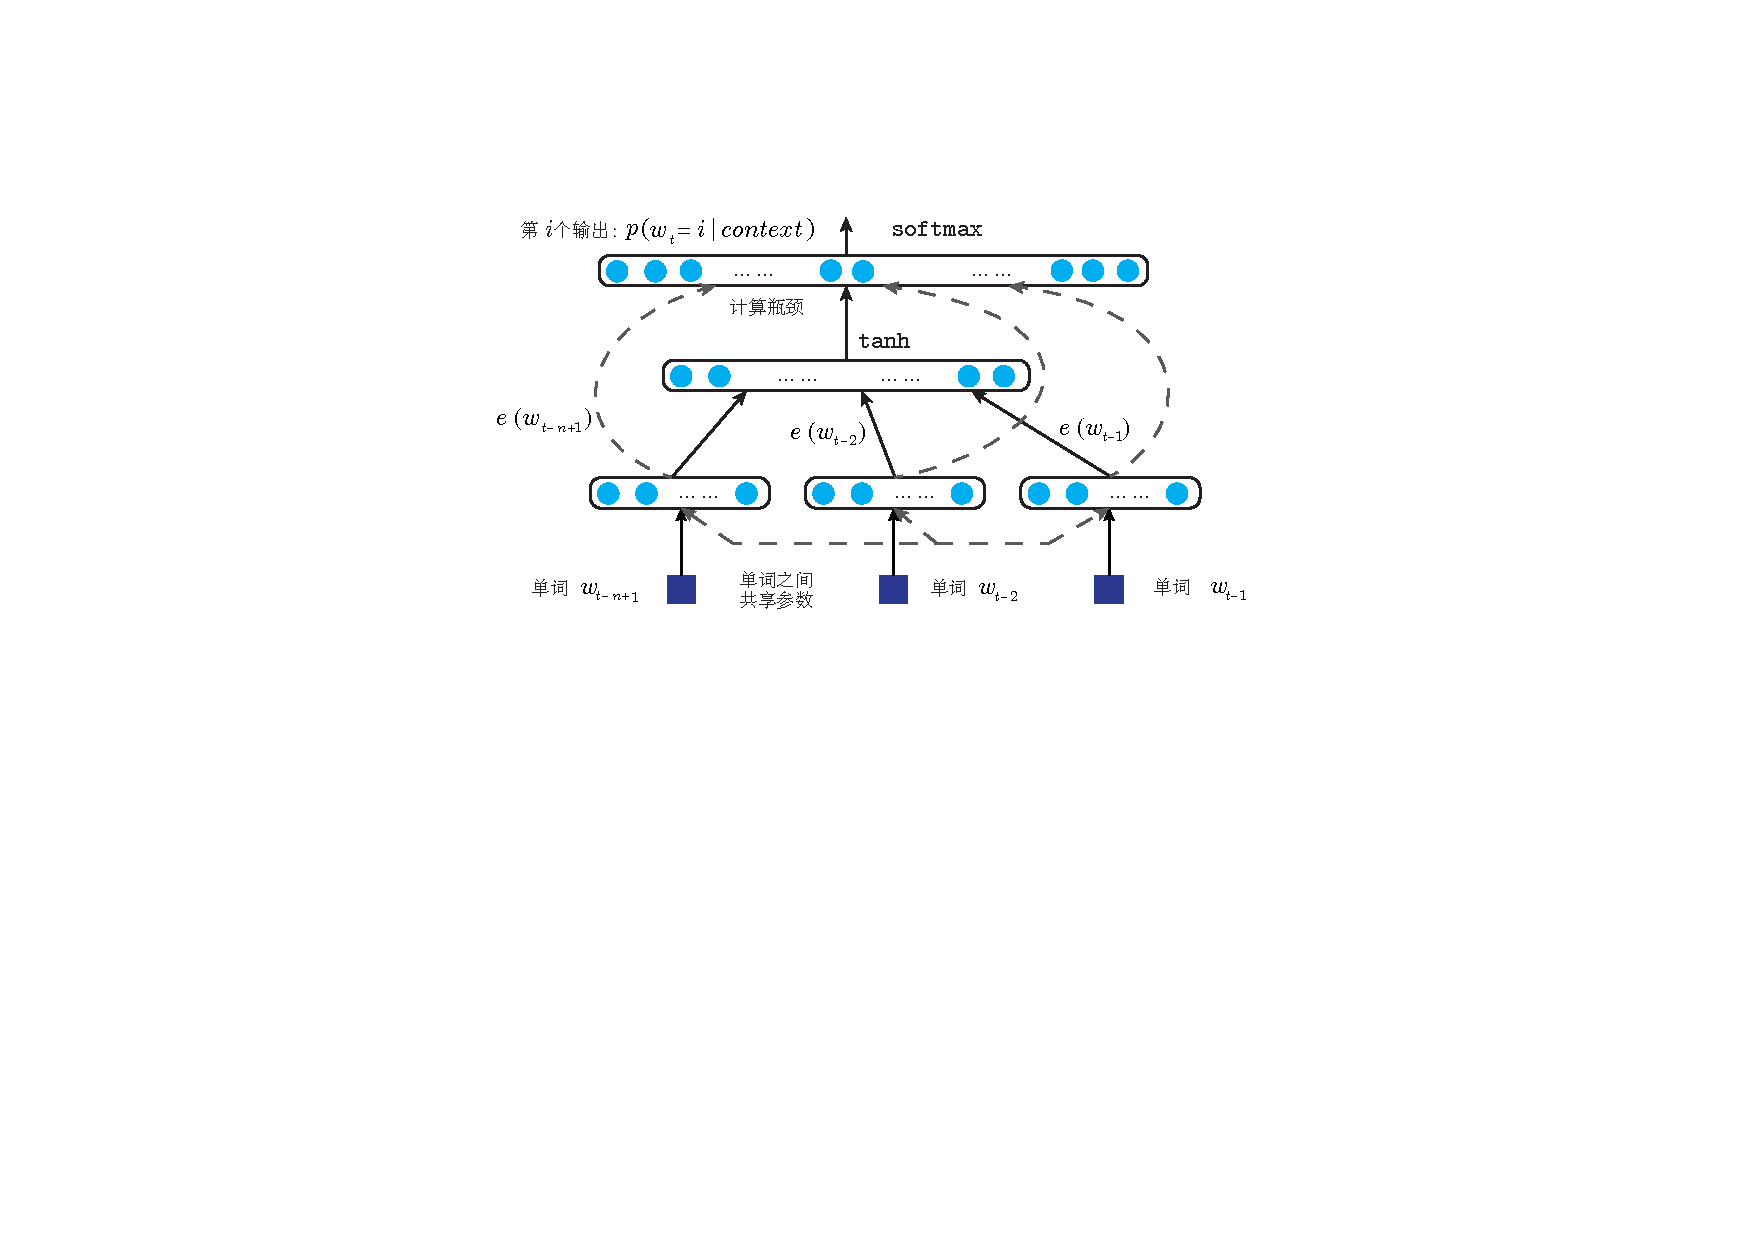
\includegraphics[width=.85\linewidth]{./figures/nplm.pdf}
  \caption{前馈神经网络语言模型}\label{fig:nplm}
\end{figure}

图~\ref{fig:nplm} 给出一个典型的采用三层前馈神经网络结构 NPLM 语言模型。其中输入层用于表征前$n$个单词的高维分布;隐藏层,表征单词的上下文信息,最后一层是输出预测层,预测下一时刻的可能出现的单词概率分布。为了解决数据稀疏问题,Bengio~等人提出拼接(Concatenation)各词的词向量作为输入,如下所示:
\begin{equation}\label{equ:we}
  x = [e(w_{i-(n-1)}), \cdots , e(w_{i-2}), e{(w_{i-1})}]
\end{equation}
模型的隐藏层$h$ 和输出层$y$可以依照下面的公式计算获得:
\begin{equation}\label{equ:nplm}
\setlength{\abovedisplayskip}{6pt}
\setlength{\belowdisplayskip}{6pt}
\begin{split}
h =& \tanh(Hx+b) \\
y =&Wx + Uh +b'
\end{split}
\end{equation}
其中参数矩阵~$H,W,U$~指代层与层之间的权重\upcite{赵林2007一种新的基于结构的神经网络规则抽取方法},参数向量~$b,b'$~均为模型中的偏置项(Bias)。如果存在$W$,那么模型能直接学习一个线性模型,需要训练的时间减少;如果不存在$W$,模型学习到非线性的网络模型,具有更好的泛化性(Generalization)。因此在后续工作中,很少有使用输入层到输出层直连边的工作,下文我们也直接忽略这一种直连的操作。假设不考虑$W$ 矩阵,整个模型计算量最大的运算,就是从隐藏层到输出层的矩阵运算$Uh$,后续的模型均有对这一矩阵乘法计算做优化。

\subsection{对数双线性语言模型}
2007 年,Mnih 和 Hinton 在神经网络语言模型(NNLM)的基础上提出了对数双线性语言模型(Log-Bilinear Language Model, LBL)~\upcite{DBLP:conf/icml/MnihH07}。LBL~模型与~NNLM~模型的区别正如它们的名字所示,其中~LBL~的模型结构是一个对数双线性结构;~NNLM~的结构不包含双线性结构,仅仅是简单的前馈网络。具体来讲,LBL 模型的代价函数为:
\begin{equation}
\setlength{\abovedisplayskip}{6pt}
\setlength{\belowdisplayskip}{6pt}
\label{equ:lbl}
\begin{split}
   &\hat r=\sum_{i=1}^{n-1}{U_i e({w_i})}, \\
   &p(w_n=w|w_{1:n-1})=\frac{\exp(\hat r^\top e(w))}{\sum_j{\exp(\hat r^\top e(w_j))}}
\end{split}
\end{equation}
其中 $\hat r$ 代表了语言模型的上下文信息,$U_i$ 指代的是对应单词的权重向量。然后基于上下文信息表示 $\hat r$ 和下一个单词的目标词汇表中所有单词 $e(w),w\in \mathcal{V}$ 的表示之间的相似度来计算下一个单词的可能的概率分布。

公式~(\ref{equ:lbl})~所描述LBL模型的代价函数与公式~(\ref{equ:nplm})~所描述~NNLM~模型的代价函数的主要区别有:1) LBL 模型中,没有非线性的激活函数$\tanh$,而由于NNLM 是非线性的神经网络结构,激活函数必不可少;2) LBL 模型中,只有一份词向量$e$,也就是说,无论一个词是作为上下文,还是作为目标词,使用的是同一份词向量。其中第二点(只有一份词向量),只在原版的LBL 模型中存在,后续的改进工作均不包含这一特点。

后来,Mnih~等人以~LBL~模型为基础,并对其所存在缺点做了一系列改进工作。其中最重要的模型有两个:逆向量语言模型(inverse vector LBL,ivLBL)~\upcite{DBLP:conf/nips/MnihK13}和层次对数双线性语言模型(Hierarchical LBL,HLBL)~\upcite{DBLP:conf/icml/MnihT12}。

\subsection{循环神经网络语言模型}
对于循环神经网络来说,它能直接对序列概率~$p(w_t | w_1,w_2,\cdots,w_{t-1})$~进行建模,而不使用公式~(\ref{equ:approx})~对其进行简化~\upcite{mikolov2012statistical,DBLP:conf/interspeech/MikolovKBCK10} 。RNNLM 模型结构如图~\ref{fig:rnnlm}~所示,它的核心方法在于其隐藏层的计算公式:
\begin{equation}
\setlength{\abovedisplayskip}{6pt}
\setlength{\belowdisplayskip}{6pt}
\label{equ:rnn}
  h_t \leftarrow  \phi(e(w_t) + U h_{t-1} +b),
\end{equation}
其中 $\phi$ 为非线性激活函数。在上述公式中,$h_t$ 表示文本中第 $t$ 个词 $w_t$ 所对应的隐藏层,该隐藏层由词向量 $e(w_t)$ 以及上一个步的隐藏层输出 $h_{t -1}$ 计算得到。隐藏层的初始状态为$h_0$,随着模型逐个读入单词:$w_1,w_2,\cdots$, 隐藏层根据公式~(\ref{equ:rnn})~被计算出来并被输出:$h_1,h_2,\cdots$ 。通过这种自身迭代更新方式,囊括了此单词前所有上文的信息,相比NPLM模型,RNNLM 理论上能学习到更丰富、更长距离的知识,也有更大的潜力达到更好的效果。最后,RNNLM 模型的输出层与NPLM 模型的输出层都采用softmax算法,两者是一致的。

\begin{figure}
  \centering
  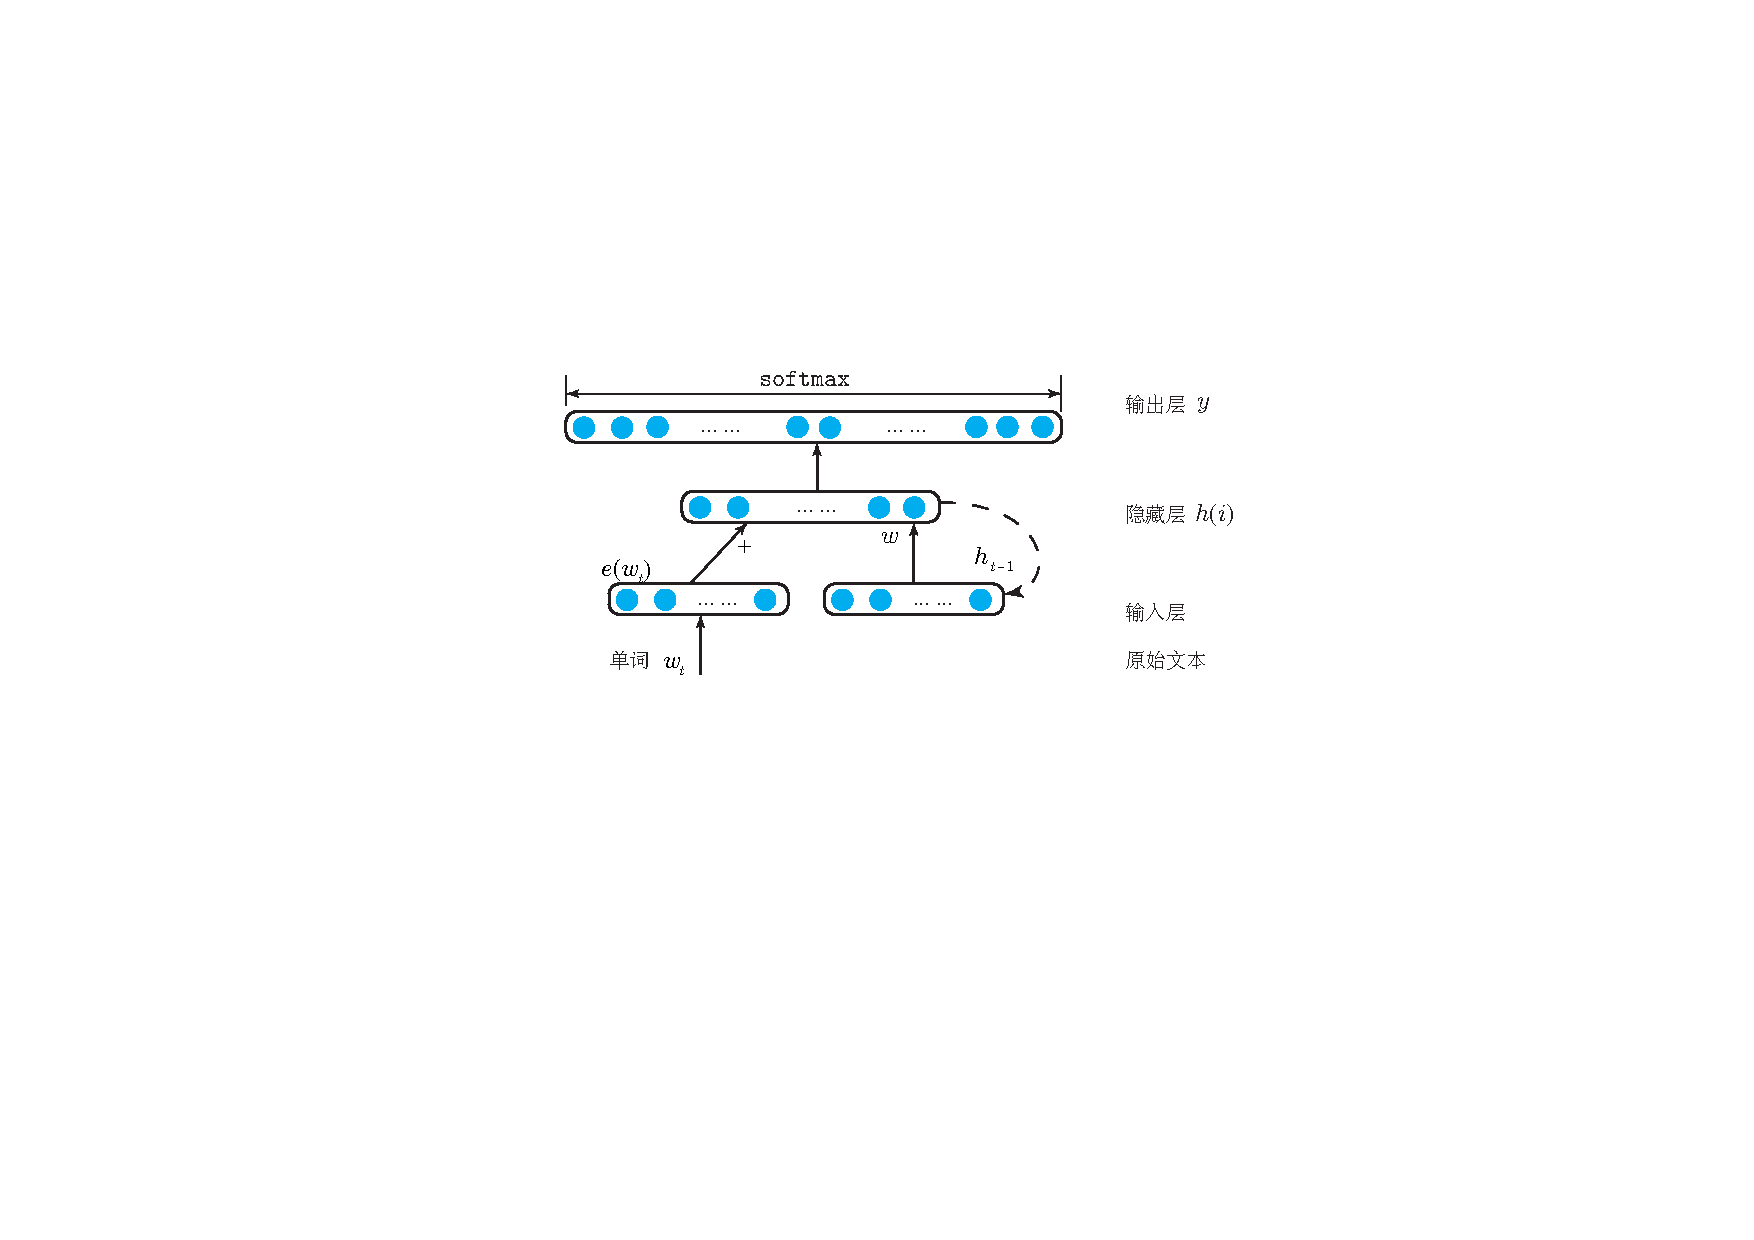
\includegraphics[width=.8\linewidth]{./figures/rnnlm.pdf}
  \caption{循环神经网络语言模型结构图}\label{fig:rnnlm}
\end{figure}


除了介绍的两种经典的建模方法,最近研究者提出可以使用带有门限机制(Gating)的RNN来防止模型的长距离依赖问题,例如长短记忆网络(Long Short-Term Memory, LSTM), 门限记忆节点(Gated Recurrent Unit, GRU)和其他网络。


\section{论文研究内容}
在历史文献当中,源词和目标词分别被称为模型的输入和输出。源词通常可以用分布式表示(Distributed Representation)来表示,称为输入词嵌入(Word Embedding),可以使用基于外部语料库的连续词袋模型(CBoW)或跳跃单词模型(Skipgram)模型来训练。而这两个模型来源于语言模型任务,并且为了在特征空间中产生可能的嵌入分布而被大大简化。另外,输出字通常表示为字索引(Indexing)或~$1-K$~编码,并且可以与softmax概率函数直接关联。

语言模型的大词表问题是目前理论应用到实际过程中必须要克服的问题,我们当然可以通过配置高性能服务器来暂时延缓该问题的后果。但是一旦应用到大数据集上,即使是目前最好的中央处理器(CPU)或者图形处理器通用计算(GPGPU),仍然需要一个多月时间才能训练完善。因此,在保证原有模型的准确率和精度的前提下,如何提高模型的训练速度是我们主要讨论和研究的内容。为此我们讨论了两个不同的内容:上下文信息建模效率和精度对比和大词表问题的优化和研究。

针对上下文信息建模手段,目前主要采用的方案有以下几种:一种是采用子词(Subword-level)或者字符级别的词(Character-level)来直接缩小词表大小;一种是通过采样技术(Sampling-based Approximation)来减少必要的训练时间;一种是通过基于分类的多元分类(class-based Hierarchical Softmax, cHSM)来加速模型和采用基于树模型的多层二元分类模型(tree-based Hierarchical Softmax, tHSM)。同时,我们还需要针对CPU 和GPGPU设备分别进行探讨。因为传统的线性运算模型在流行的GPGPU并行运算方案中并不适用,所有需要结合不同的运算设备分别讨论可行的方案。

在本节中,我们将这个目标词表示扩展到一个分层的形式,使它们适配基于类和基于树的分层概率计算。首先,我们提出了一个在分层结构上建模参数的字编码方案。因此,考虑到~GPGPU~上的并行吞吐性能,我们推导出紧凑的代价函数及其梯度。同时,类或树上的单词分布对其性能有很大的影响,应该在训练阶段之前定义,这些动态交换算法在训练过程中改变了单词群或子树结构在这个研究中。我们采用了几个分层聚类和词汇分割策略,用统计,句法和语义知识来初始化其结构,以达到一个稳定和可以预期的性能。而且,在推理过程中,不同于传统的softmax情况,得到最好的候选者自然是可行的,层次推理不能直接用 softmax 方法来实现。我们讨论基于树和基于类的搜索策略的两种不同的推理情况:1)打分:输出给定序列的概率;2)排序   :在给定的上下文中获取得分最高的一个候选单词。
\section{论文的组织结构}
\textbf{第一章:}``绪论'',主要介绍了本论文的研究背景和意义,另外简要说明了语言模型的发展历史以及本文的主要工作,并对本文的组织架构进行了说明。

\textbf{第二章:}``相关技术介绍'',对历史上的各个学术流派在语言模型的任务上相关工作进行了介绍。

\textbf{第三章:}``并行树状概率模型'',介绍了基于二叉树的层次概率模型,并比较了传统树状模型的差一点。同时还研究了在推理测试阶段,二叉树层次概率模型能应用的策略,以保证实际测试结果性能和效率。


\textbf{第四章:}``并行分类层次概率模型'',介绍基于分类的层次概率模型,并分析了词表非均匀划分所产生的后果,进而探讨了类别不均匀问题所带来的影响以及相关解决策略。最后探讨了在测试阶段,语言模型的任务需求和分类层次概率模型相应的解决算法。

\textbf{第五章:}``语言模型实验及实验结果分析'',实证研究了本论文提出的并行层次概率模型的实际效果,并和其他算法在各个指标维度上进行了比较和分析。

最后结论部分,总结了全论文的贡献和工作,并提出了未来的工作方向,同时撰写了结束语。



